\documentclass[a4paper, twocolumn, 9pt]{article}

% --- Essential Packages ---
\usepackage[utf8]{inputenc}
\usepackage[T1]{fontenc}
\usepackage{amsmath, amssymb}
\usepackage{graphicx}
\usepackage{booktabs}
\usepackage[columnsep=0.7cm, top=2cm, bottom=2cm, left=1.5cm, right=1.5cm]{geometry}
\usepackage{hyperref}

% --- Custom Math Commands ---
\newcommand{\dpo}{\text{DPO}}
\newcommand{\DPO}{\text{DPO}}

% --- Title Information ---
\title{\vspace{-1.5cm}\textbf{Steerability–Robustness Tradeoff in Language Models via Direct Preference Optimization ($\dpo$)}\vspace{0.5cm}}

\author{
    Mahmoud Zahran$^1$ \quad Yahya Al Malallah$^1$ \quad Kumail Alhamoud$^2$ \\
    \small $^1$King Abdullah University of Science and Technology (KAUST) \quad
    $^2$Massachusetts Institute of Technology (MIT) \\
    \small \texttt{mahmoud.zahran@kaust.edu.sa}, \texttt{yahya.almalallah@kaust.edu.sa}, \texttt{kumail@mit.edu}
}

\date{December 4, 2025}

% -------------------------------------------------------------
\begin{document}
\maketitle

% -------------------------------------------------------------
\begin{abstract}
Safety alignment, often implemented via Direct Preference Optimization (DPO), is widely assumed to impose a uniform capability tax: models become safer but less capable across the board. We systematically test this assumption by performing a controlled DPO study across five regularization parameter ($\beta$) settings on two distinct open-weight models, Llama~3.1-8B and Qwen~2.5-7B. We evaluate safety using GPT-4o on 520 AdvBench prompts and capabilities on 1{,}000 MMLU (factual knowledge) and 500 GSM8K (complex reasoning) problems.

We confirm that DPO dramatically improves safety, increasing refusal rates from 22.3\% to 85.2\% for Llama and from 53.3\% to 100.0\% for Qwen in the strongest configurations. Crucially, the capability cost is asymmetric and model-dependent. Factual knowledge (MMLU) remains remarkably stable for both models, with changes within roughly $\pm 2$ points, indicating that safety DPO does not impose a significant knowledge tax. In sharp contrast, complex reasoning (GSM8K) proves catastrophically vulnerable in Qwen: accuracy plummets from 78.8\% to 25.2\% at $\beta=0.01$, while Llama’s reasoning remains largely unaffected. Increasing $\beta$ partially recovers Qwen’s reasoning (up to 47.6\%) while maintaining strong safety (93.5\% refusal).

Our results demonstrate that the DPO capability tax is not uniform: it primarily targets complex reasoning while leaving factual knowledge intact. We conclude that $\beta$ must be tuned not only for safety, but also to manage the fragility of reasoning circuits in safety-aligned models, especially in math- and logic-heavy applications.\footnote{Code and data available at \url{https://github.com/mahmoudzahran01/-steerability-robustness-dpo}}
\end{abstract}



% -------------------------------------------------------------
\section{Introduction}

Can we make language models safer without making them dumber?
As LLMs are deployed in increasingly sensitive settings, this question sits at the
center of practical alignment. Safety interventions such as supervised safety
fine-tuning, RLHF~\cite{rlhf}, and rule-based filters reliably reduce harmful outputs,
but practitioners frequently report unwanted side effects: models over-refuse benign
queries, hallucinate "I cannot help with that" in harmless contexts, or exhibit
drops in reasoning and knowledge benchmarks. These behaviors motivate the widely held
concern that safety alignment inevitably incurs a \emph{capability tax}.

Direct Preference Optimization (DPO)~\cite{dpo} has become a popular alternative to RLHF,
offering a simpler alignment pipeline by directly optimizing over paired preference
data under a KL-regularized objective. DPO is now central to many open-source
alignment frameworks and is commonly paired with large safety preference datasets such
as PKU-SafeRLHF~\cite{pku-saferlhf}. Despite its widespread adoption, the field still lacks
a systematic understanding of how safety DPO affects model capabilities, particularly
across different model families and alignment strengths. Most existing reports evaluate
a single configuration, leaving open the central question:
\emph{Does DPO make models safer at the cost of capability, or can it achieve safety
without the tax?}

We address this question empirically through a controlled, multi-model study.
We evaluate two representative open-weight models with sharply contrasting
pretrained safety profiles:
Llama~3.1-8B, which is relatively permissive after instruction tuning
(22.3\% refusal on AdvBench), and Qwen~2.5-7B, which is substantially safer by
default (53.3\% refusal). Using the same strictly filtered preference dataset, we
apply DPO across five regularization strengths ($\beta \in \{0.01, 0.05, 0.1, 0.5, 1.0\}$)
to map how safety and capability evolve under progressively stronger alignment.

\begin{figure}[t]
    \centering
    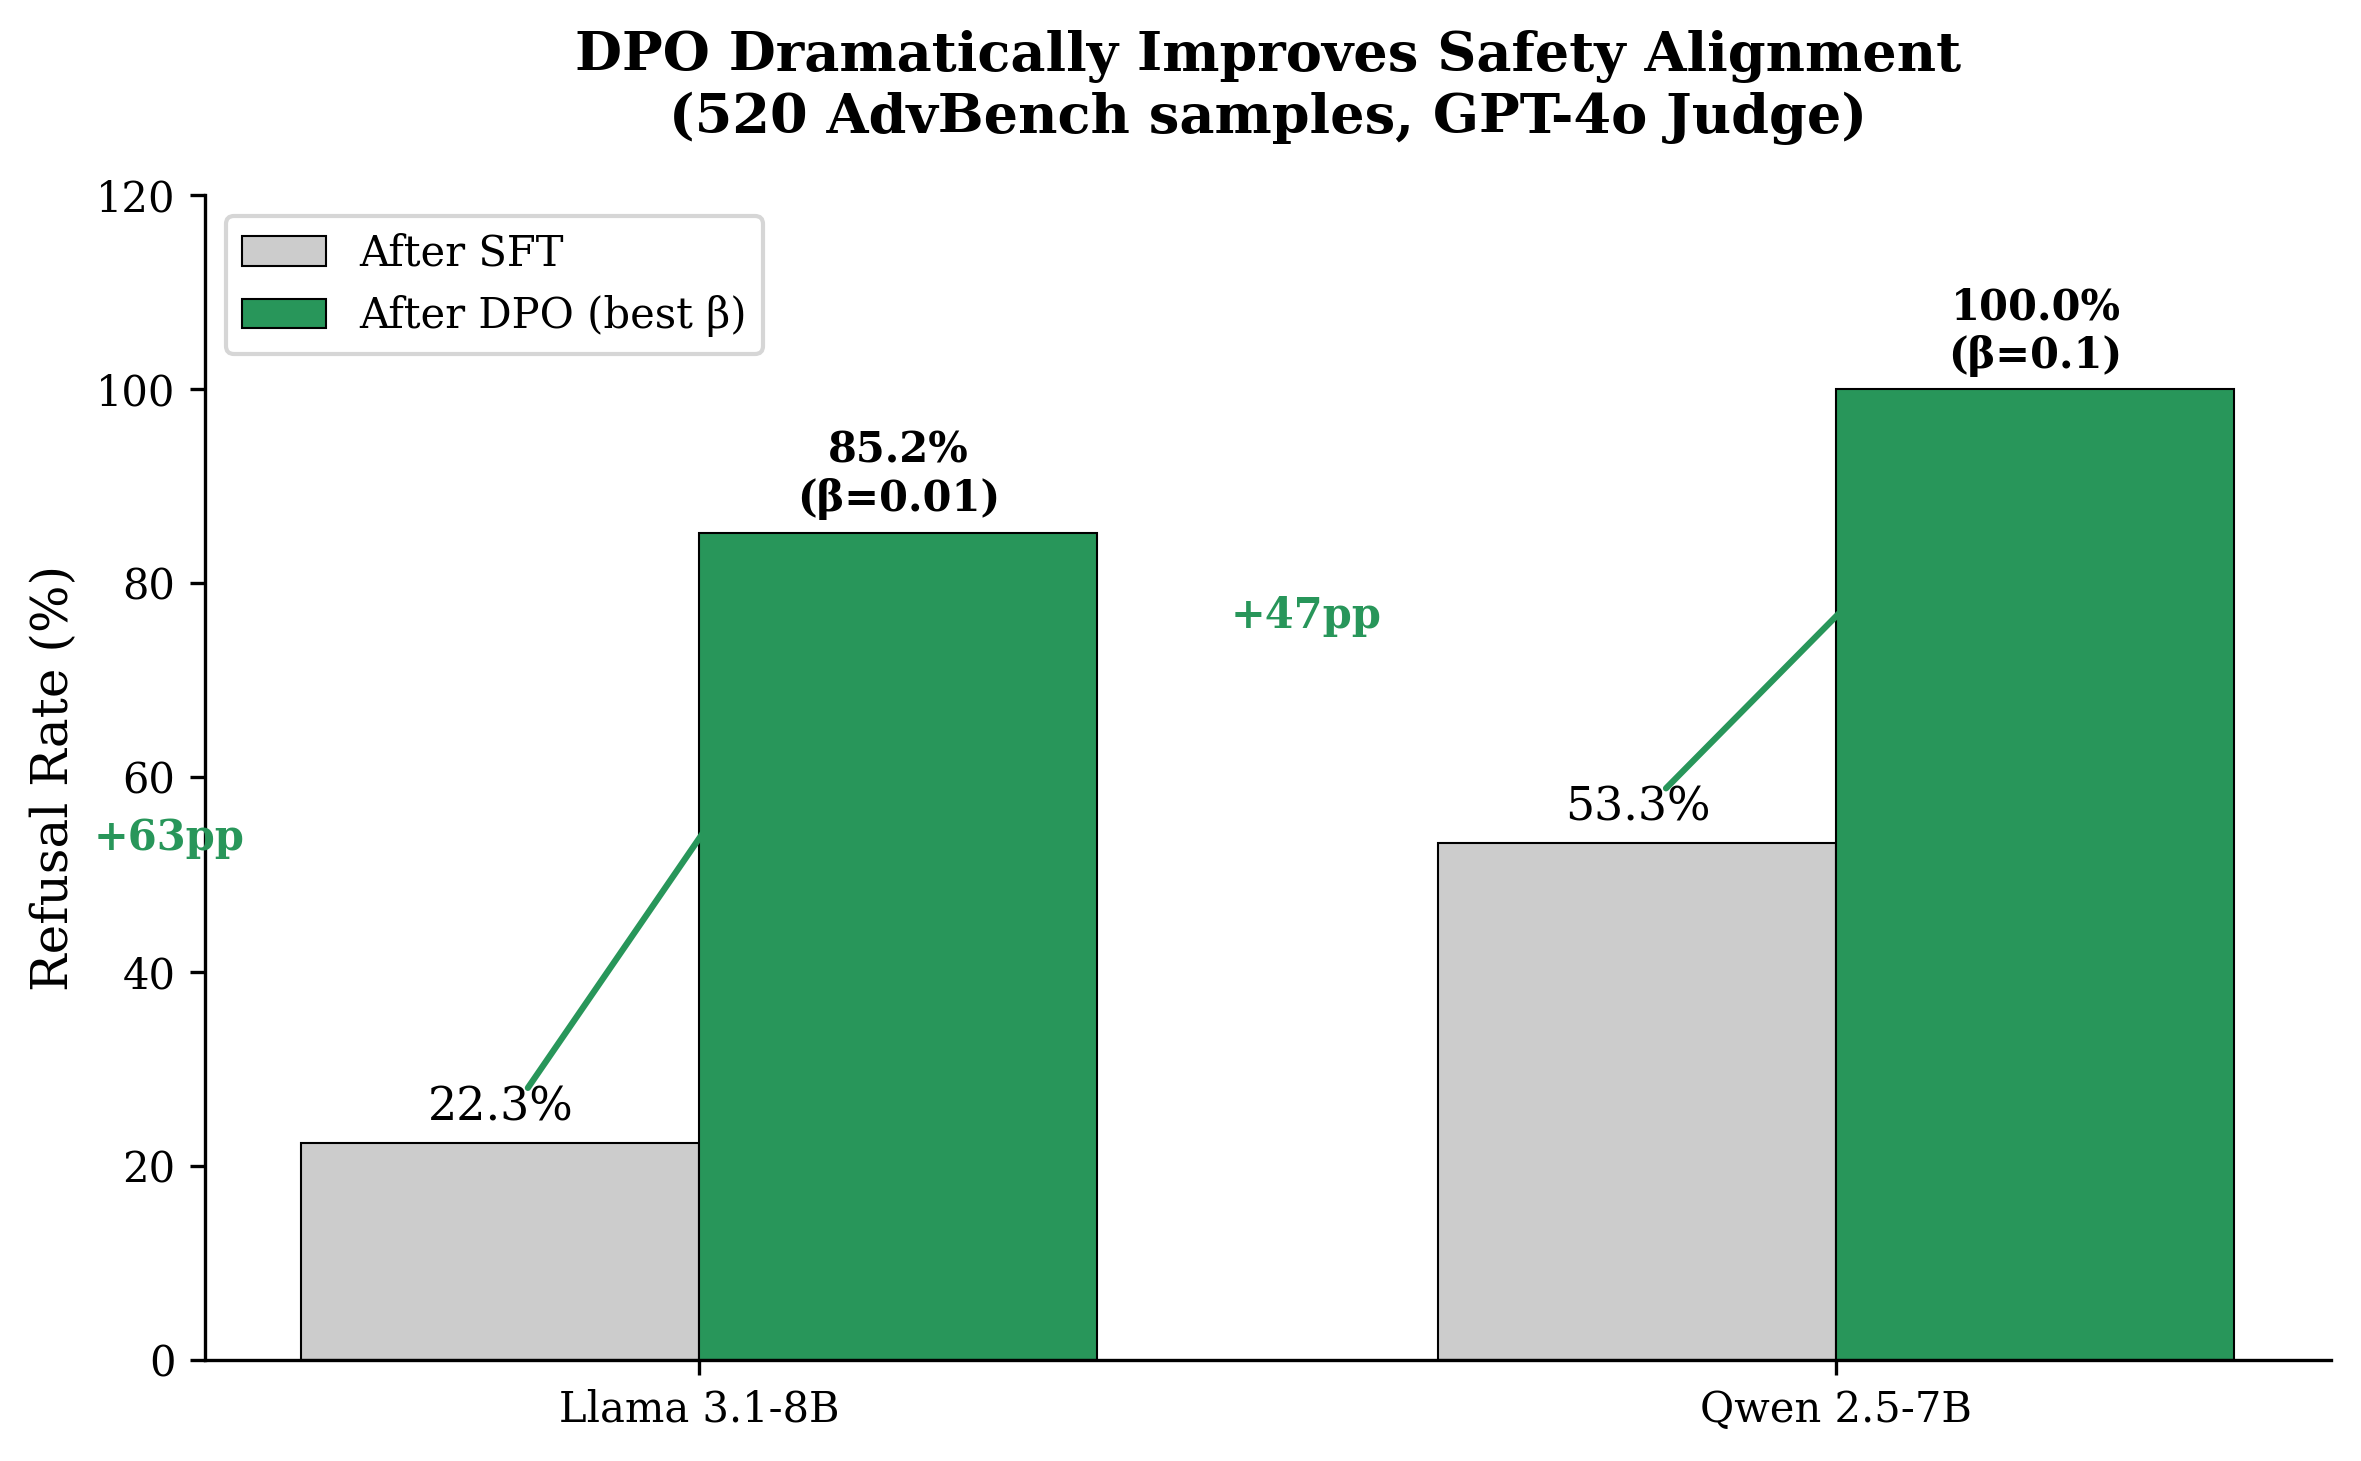
\includegraphics[width=0.9\linewidth]{fig1_safety_improvement.png}
    \caption{\textbf{DPO dramatically improves safety alignment.}
    Refusal rates before (SFT) and after the best-performing DPO configuration
    for each model.}
    \label{fig:intro_safety}
\end{figure}

Figure~\ref{fig:intro_safety} previews our main finding: DPO reliably and
substantially increases safety for both models, pushing them into a high-safety regime.
However, the capability cost is uneven.
While Llama maintains stable performance on both MMLU and GSM8K across all
settings, Qwen experiences a steep degradation in GSM8K accuracy under the
strongest safety alignment, revealing a vulnerability of complex reasoning to
aggressive preference-based alignment.

Our contributions are:
\begin{itemize}
    \item We conduct a controlled empirical study of DPO-based safety alignment across
          two distinct model families and five alignment strengths.
    \item We show that DPO reliably increases safety for both models, but that the
          capability tax is task- and model-dependent: factual knowledge
          remains stable, Llama's reasoning is largely preserved, while Qwen's
          reasoning degrades sharply under aggressive alignment.
    \item We characterize the resulting safety--capability frontier and identify
          operating points that balance high safety with acceptable reasoning
          performance.
    \item We provide practical guidance: tuning $\beta$ is crucial not only for
          safety but also for mitigating disproportionate losses in reasoning-heavy
          downstream applications.
\end{itemize}


% -------------------------------------------------------------
\section{Related Work}

\paragraph{Safety Alignment and the Capability Tax.}
The post-training phase is critical for aligning LLMs with human values.
Early alignment methods include supervised fine-tuning (SFT) on curated
instruction datasets and reinforcement learning from human feedback (RLHF)~\cite{rlhf}.
While these interventions reliably reduce harmful outputs and increase helpfulness,
they often introduce undesirable side effects. A central concern is the
\emph{alignment tax}---or \emph{capability tax}---introduced by Askell et al.~\cite{askell2021alignment},
which refers to the degradation of general capabilities as a consequence of safety tuning.
This degradation frequently manifests as \emph{over-refusal}, where models reject even
benign or creative requests that superficially resemble unsafe prompts~\cite{llm-overrefusal}.
Recognizing the growing prevalence of over-generalized safety behavior, several benchmarks
such as OR-Bench~\cite{orbench} and FalseReject~\cite{falsereject} have been developed to
quantify the reliability impact of miscalibrated refusals.

\paragraph{Preference Optimization and Direct Preference Optimization (DPO).}
In response to the complexity and instability of RLHF pipelines, reward-model-free
preference optimization methods have emerged as simpler and more robust alternatives.
Direct Preference Optimization (DPO)~\cite{dpo} optimizes directly over human preference
pairs using a KL-regularized objective, avoiding the need to fit an explicit reward
model. The DPO objective can be derived from the policy-optimization perspective of PPO,
linking preference learning to a principled trust-region framework. Because of its
simplicity, stability, and strong empirical performance, DPO has become a standard
component of many open-weight alignment pipelines and is frequently trained on large,
curated safety preference datasets such as PKU-SafeRLHF~\cite{pku-saferlhf}.
However, despite its widespread adoption, the influence of its key regularization
hyperparameter $\beta$ on capability preservation---particularly in reasoning-heavy tasks---
remains poorly understood.

\paragraph{Systematic Tradeoff Analysis.}
Recent work highlights that model safety behavior varies dramatically across architectures
and pretraining regimes, with similarly sized open-weight models exhibiting widely
different baseline refusal rates and robustness to adversarial prompts.
While several studies have examined mechanisms behind over-refusal and capability loss~\cite{llm-overrefusal},
there is limited systematic analysis of how preference-based alignment reshapes the
safety--capability landscape across model families.
In particular, prior work rarely sweeps the alignment strength ($\beta$) or compares
models with divergent pretrained safety priors under equivalent DPO pipelines.
Our work fills this gap by quantifying how safety DPO affects both factual knowledge
and complex reasoning across two distinct model families, revealing that the capability
tax is neither inevitable nor uniform, but task- and model-dependent.


% -------------------------------------------------------------
\section{Methodology}
\label{sec:method}

\subsection{Model Selection and Baselines}

We study two representative mid-sized open-weight LLMs whose pretrained safety
profiles differ substantially:

\begin{itemize}
\item \textbf{Llama 3.1-8B}~\cite{llama3}: a general-purpose model with a relatively
      permissive safety posture after instruction tuning, exhibiting a refusal rate
      of 22.3\% on AdvBench in our evaluation.
\item \textbf{Qwen 2.5-7B}~\cite{qwen2.5}: a model with stronger built-in safety priors,
      yielding a substantially higher SFT refusal rate of 53.3\%.
\end{itemize}

Both models are used in their instruction-tuned variants and are further adapted
using parameter-efficient fine-tuning (PEFT) to ensure comparability across DPO runs.

\subsection{Training Pipeline}

To ensure consistent initialization, all experiments follow the same two-stage
pipeline:
\[
\text{Base Model} \;\rightarrow\; \text{SFT (Alpaca)} \;\rightarrow\; \text{DPO (PKU-SafeRLHF)}.
\]

\paragraph{Supervised fine-tuning (SFT).}
We first fine-tune each base model on the Alpaca 52k dataset using LoRA adapters
(rank 64, $\alpha=16$), with a learning rate of $1\times 10^{-4}$ and sequence length 2048.
This establishes a uniform instruction-following baseline before applying safety
alignment.

\paragraph{Direct Preference Optimization (DPO).}
DPO~\cite{dpo} optimizes the policy $\pi_\theta$ directly on preference pairs without
fitting an explicit reward model. The loss is:
\begin{align}
\mathcal{L}_{\text{DPO}} = -\mathbb{E}\Big[ \log \sigma \big(
& \beta \log \tfrac{\pi_\theta(y_w|x)}{\pi_{\text{ref}}(y_w|x)} \nonumber \\[-2pt]
& - \beta \log \tfrac{\pi_\theta(y_l|x)}{\pi_{\text{ref}}(y_l|x)} \big) \Big]
\label{eq:dpo}
\end{align}
where $(x, y_w, y_l) \sim \mathcal{D}$ are prompts with preferred/dispreferred responses, $\pi_{\text{ref}}$ is the SFT reference, and $\beta$ controls divergence from it.

We apply DPO using LoRA adapters (rank 64), training for two epochs on the filtered
preference dataset with a learning rate of $5\times10^{-5}$ and batch size 64.
To study how alignment strength affects safety and capability, we sweep over
\[
\beta \in \{0.01,\, 0.05,\, 0.1,\, 0.5,\, 1.0\}.
\]
Lower $\beta$ values place greater weight on the preference signal (stronger
alignment), while higher values constrain the policy closer to the SFT baseline.

\subsection{Safety Preference Dataset}

We construct a high-confidence safety preference dataset from
PKU-SafeRLHF~\cite{pku-saferlhf} using strict filtering to maximize the clarity of
the safety signal. A pair is retained only if:

\begin{itemize}
\item exactly one response is labeled safe,
\item the chosen/rejected labels are internally consistent,
\item both responses are non-empty, and
\item the preference direction is unambiguous.
\end{itemize}

This yields approximately 18{,}000 high-quality preference pairs.
Under this construction, DPO primarily learns to replace unsafe completions with
safe alternatives rather than optimizing stylistic preferences or helpfulness.

\subsection{Evaluation Benchmarks}

\paragraph{Safety.}
We measure safety using AdvBench~\cite{advbench}, a dataset of 520 adversarial prompts
targeting categories such as weapons, self-harm, violent crime, cyber attacks, and
chemical/biological threats. For each prompt, the model generates a response that is
classified as a refusal or non-refusal.

\paragraph{Capabilities.}
Capabilities are assessed using two standard zero-shot benchmarks:
\begin{itemize}
\item \textbf{MMLU}~\cite{mmlu}: 1{,}000 questions spanning 57 academic subjects,
      probing factual knowledge and broad reasoning.
\item \textbf{GSM8K}~\cite{gsm8k}: 500 grade-school math problems requiring
      multi-step numerical reasoning.
\end{itemize}

\paragraph{LLM-as-judge for refusal detection.}
To obtain consistent refusal labels, we employ GPT-4o as an LLM judge. The judge is
prompted to identify whether a response constitutes a refusal and to verify that no
actionable harmful content is present. This avoids brittle refusal heuristics and
provides robust, high-quality safety annotations across all model configurations.

\subsection{Infrastructure}

All fine-tuning experiments are conducted on NVIDIA A100 80GB GPUs using
\texttt{bfloat16} precision and PEFT-based LoRA adapters.
Evaluation is parallelized across multiple SLURM jobs, and all prompt–response pairs
and judge labels are logged for reproducibility.


% -------------------------------------------------------------
\section{Experiments and Results}

We now present our empirical findings on the safety--capability frontier induced by DPO.
Our analysis centers on three questions:
(1) Does DPO reliably increase safety across models with different initial safety profiles?
(2) Does DPO preserve capabilities, or does it introduce a capability tax?
(3) How do alignment strength ($\beta$) and model choice shape the resulting
safety--capability tradeoff?

\subsection{Overall Safety and Capability Behavior}

Table~\ref{tab:main_results} summarizes the performance of both model families
across five DPO configurations, reporting refusal rates on AdvBench and accuracy
on MMLU and GSM8K.

\begin{table}[t]
\centering
\caption{\textbf{Expanded safety--capability results} (520 AdvBench, 1{,}000 MMLU, 500 GSM8K).
Refusal is AdvBench refusal rate (higher = safer). MMLU and GSM8K are accuracy (higher = better).}
\label{tab:main_results}
\begin{tabular}{lccc}
\toprule
Model \& Stage          & Refusal (\%) & MMLU (\%) & GSM8K (\%) \\
\midrule
Llama SFT         & 22.3 & \textbf{50.9} & \textbf{12.4} \\
Llama $\beta=0.01$& \textbf{85.2} & 49.3 & \textbf{12.4} \\
Llama $\beta=0.05$& 79.0 & 49.9 & 11.8 \\
Llama $\beta=0.1$ & 78.1 & 50.2 & 11.4 \\
Llama $\beta=0.5$ & 68.5 & 50.8 & 11.8 \\
Llama $\beta=1.0$ & 66.2 & 50.2 & 11.6 \\
\midrule
Qwen SFT         & 53.3 & 68.0 & \textbf{78.8} \\
Qwen $\beta=0.01$& 99.8 & 66.6 & 25.2 \\
Qwen $\beta=0.05$& 99.8 & 67.5 & 26.2 \\
Qwen $\beta=0.1$ & \textbf{100.0} & \textbf{68.3} & 28.6 \\
Qwen $\beta=0.5$ & 96.2 & 68.1 & 44.4 \\
Qwen $\beta=1.0$ & 93.5 & 68.1 & 47.6 \\
\bottomrule
\end{tabular}
\end{table}

Two key patterns emerge.

First, \textbf{DPO consistently and substantially increases safety} for both models.
Llama's refusal rate rises from 22.3\% (SFT) to 85.2\% at $\beta=0.01$,
a gain of over 60 percentage points.
Qwen's refusal increases from 53.3\% to 93.5--100\% across all DPO settings,
placing it in a near-fully aligned regime on AdvBench.

Second, \textbf{the capability cost is asymmetric across tasks and models}.
For both families, MMLU accuracy remains remarkably stable, shifting by at most
$\pm 2$ points.
Llama's GSM8K accuracy also stays near its SFT baseline across all $\beta$ values.
In stark contrast, Qwen's GSM8K accuracy collapses from 78.8\% (SFT)
to 25--29\% at low $\beta$ (0.01--0.1), and only partially recovers to 44--48\%
at higher $\beta$ (0.5--1.0).
This reveals a \emph{severe, reasoning-specific capability tax} for Qwen,
even as its factual knowledge remains intact.

\subsection{Safety--Capability Frontier}

Figure~\ref{fig:frontier} plots MMLU accuracy against AdvBench refusal rate for every
configuration, illustrating the tradeoff in the "knowledge vs.\ safety" plane.

\begin{figure}[t]
    \centering
    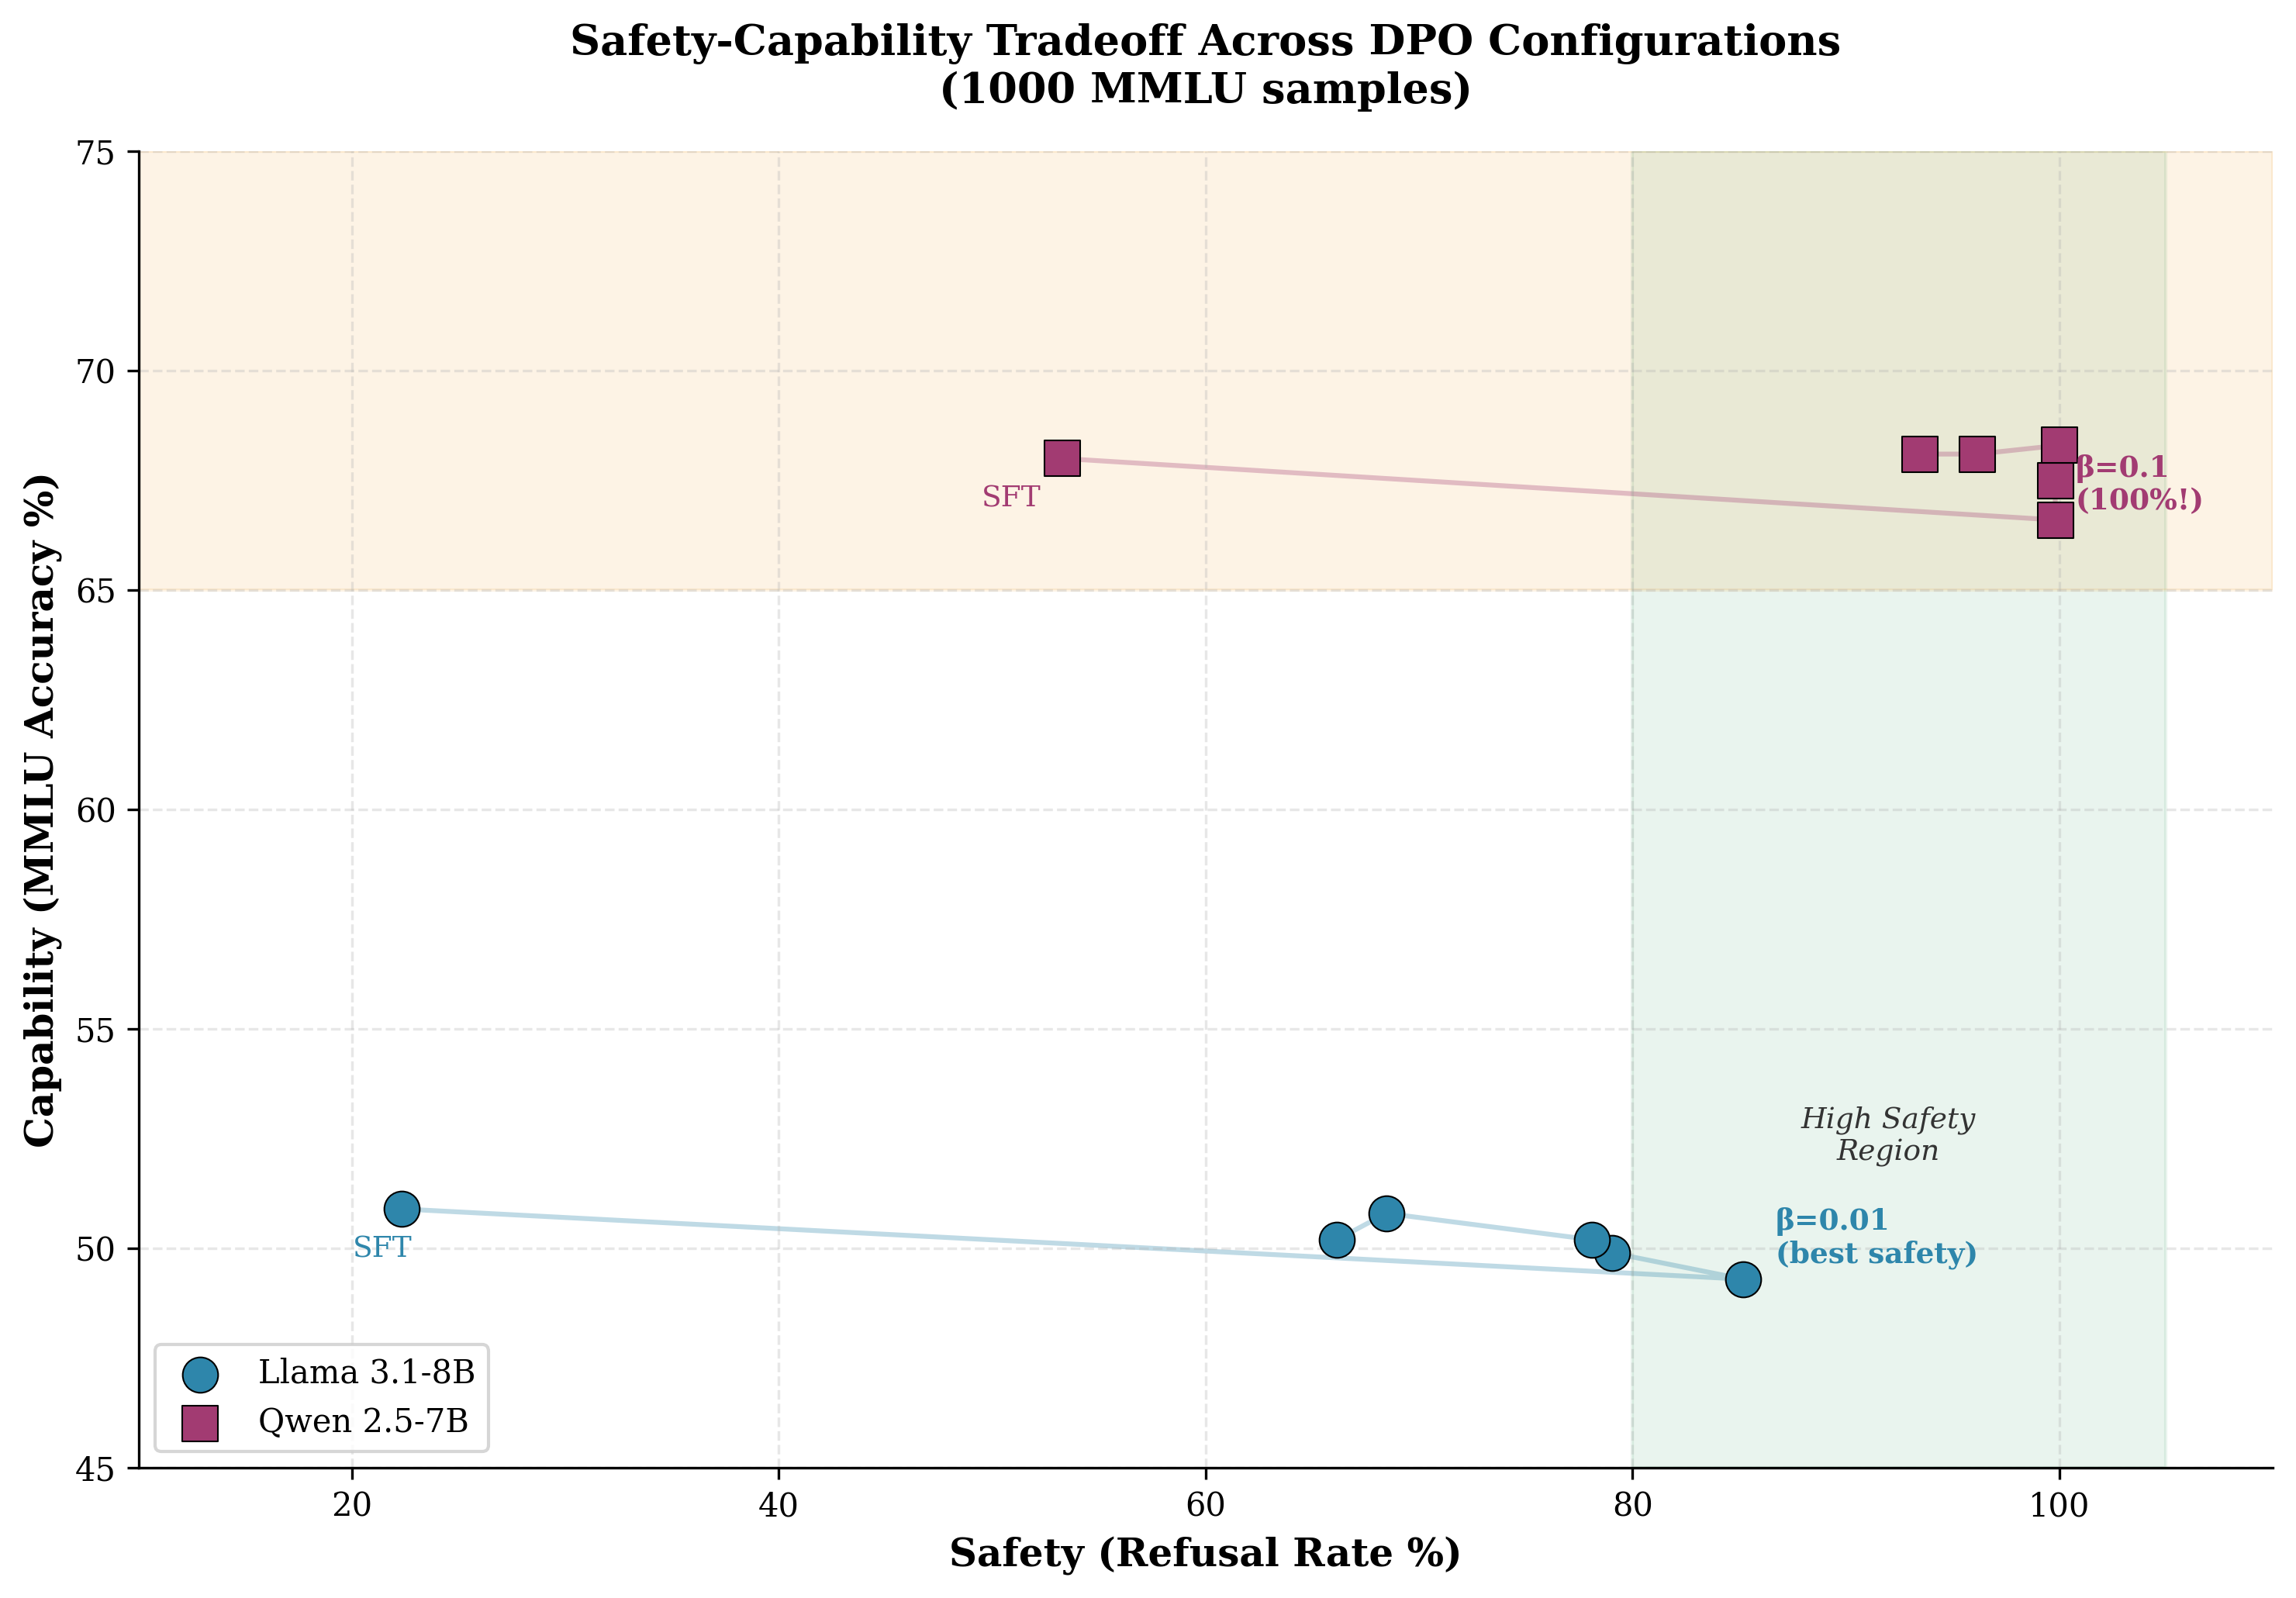
\includegraphics[width=0.95\linewidth]{fig2_safety_capability_tradeoff.png}
    \caption{\textbf{Safety--capability frontier (MMLU vs.\ AdvBench refusal).}
    Both models move into a high-safety region while maintaining near-constant MMLU,
    suggesting that factual knowledge is largely unaffected by DPO.}
    \label{fig:frontier}
\end{figure}

Both Llama and Qwen show a favorable frontier in this space:
safety increases dramatically with almost no change in MMLU.
From a knowledge perspective, DPO appears to deliver ``safety for free.''

However, this projection hides the degradation in reasoning.
When examining GSM8K (not shown here), Qwen's frontier bends sharply downward
for low $\beta$ values, revealing a steep safety--reasoning tradeoff that does not
appear in the MMLU dimension.

\subsection{Capability Preservation and Degradation}

For Llama, DPO improves safety without meaningfully altering its performance on
either benchmark (Table~\ref{tab:main_results}). We note that Llama's GSM8K baseline is low ($\sim$12\%), suggesting limited
math reasoning ability after SFT; consequently, the stability we observe may partly reflect
a floor effect rather than robustness of reasoning circuits.
For Qwen, the picture is different:
MMLU remains strong across all configurations, but GSM8K suffers catastrophic
degradation under aggressive alignment (low $\beta$), as shown in Figure~\ref{fig:summary}(b),
reflecting strong entanglement between safety training and Qwen's reasoning mechanisms.

These results highlight that \textbf{safety alignment effects are architecture-dependent}:
reasoning may be far more fragile in some models than others.

\subsection{Alignment Strength and the Safety--Reasoning Tradeoff}

The DPO hyperparameter $\beta$ controls the balance between the preference-learning
signal and the KL constraint, and therefore directly governs the tradeoff between
safety and reasoning ability.

\begin{itemize}
\item \textbf{Low $\beta$ (0.01--0.1).}
      This regime produces the strongest safety alignment, with Qwen reaching
      99.8--100.0\% refusal. MMLU remains stable, but GSM8K accuracy collapses to
      25--29\%, indicating that aggressive preference weighting induces a substantial
      reasoning-specific capability tax.

\item \textbf{Intermediate $\beta$ (0.5--1.0).}
      Here, the KL constraint exerts stronger influence, keeping the learned policy
      closer to the SFT model. Safety remains high (e.g., 93.5\% refusal for Qwen at
      $\beta=1.0$), while GSM8K partially recovers to 44--48\%. This regime represents
      a more balanced alignment configuration: safety improves significantly while
      limiting degradation in multi-step reasoning.

\end{itemize}

Notably, Llama exhibits stable behavior across the entire $\beta$ sweep, suggesting
that its reasoning mechanisms are less sensitive to safety alignment.
Overall, $\beta$ functions as a controllable parameter for navigating the
safety--reasoning tradeoff, and the appropriate setting depends on how much reasoning
performance practitioners are willing to exchange for additional safety.


% -------------------------------------------------------------
\section{Discussion}
\label{sec:discussion}

We now interpret our results through three lenses:
(1) the contrasting behavior of the two model families and the role of pretrained safety,
(2) what our findings imply about the structure of the safety--capability tradeoff, and
(3) practical considerations for using DPO as a safety alignment method.

\begin{figure}[t]
    \centering
    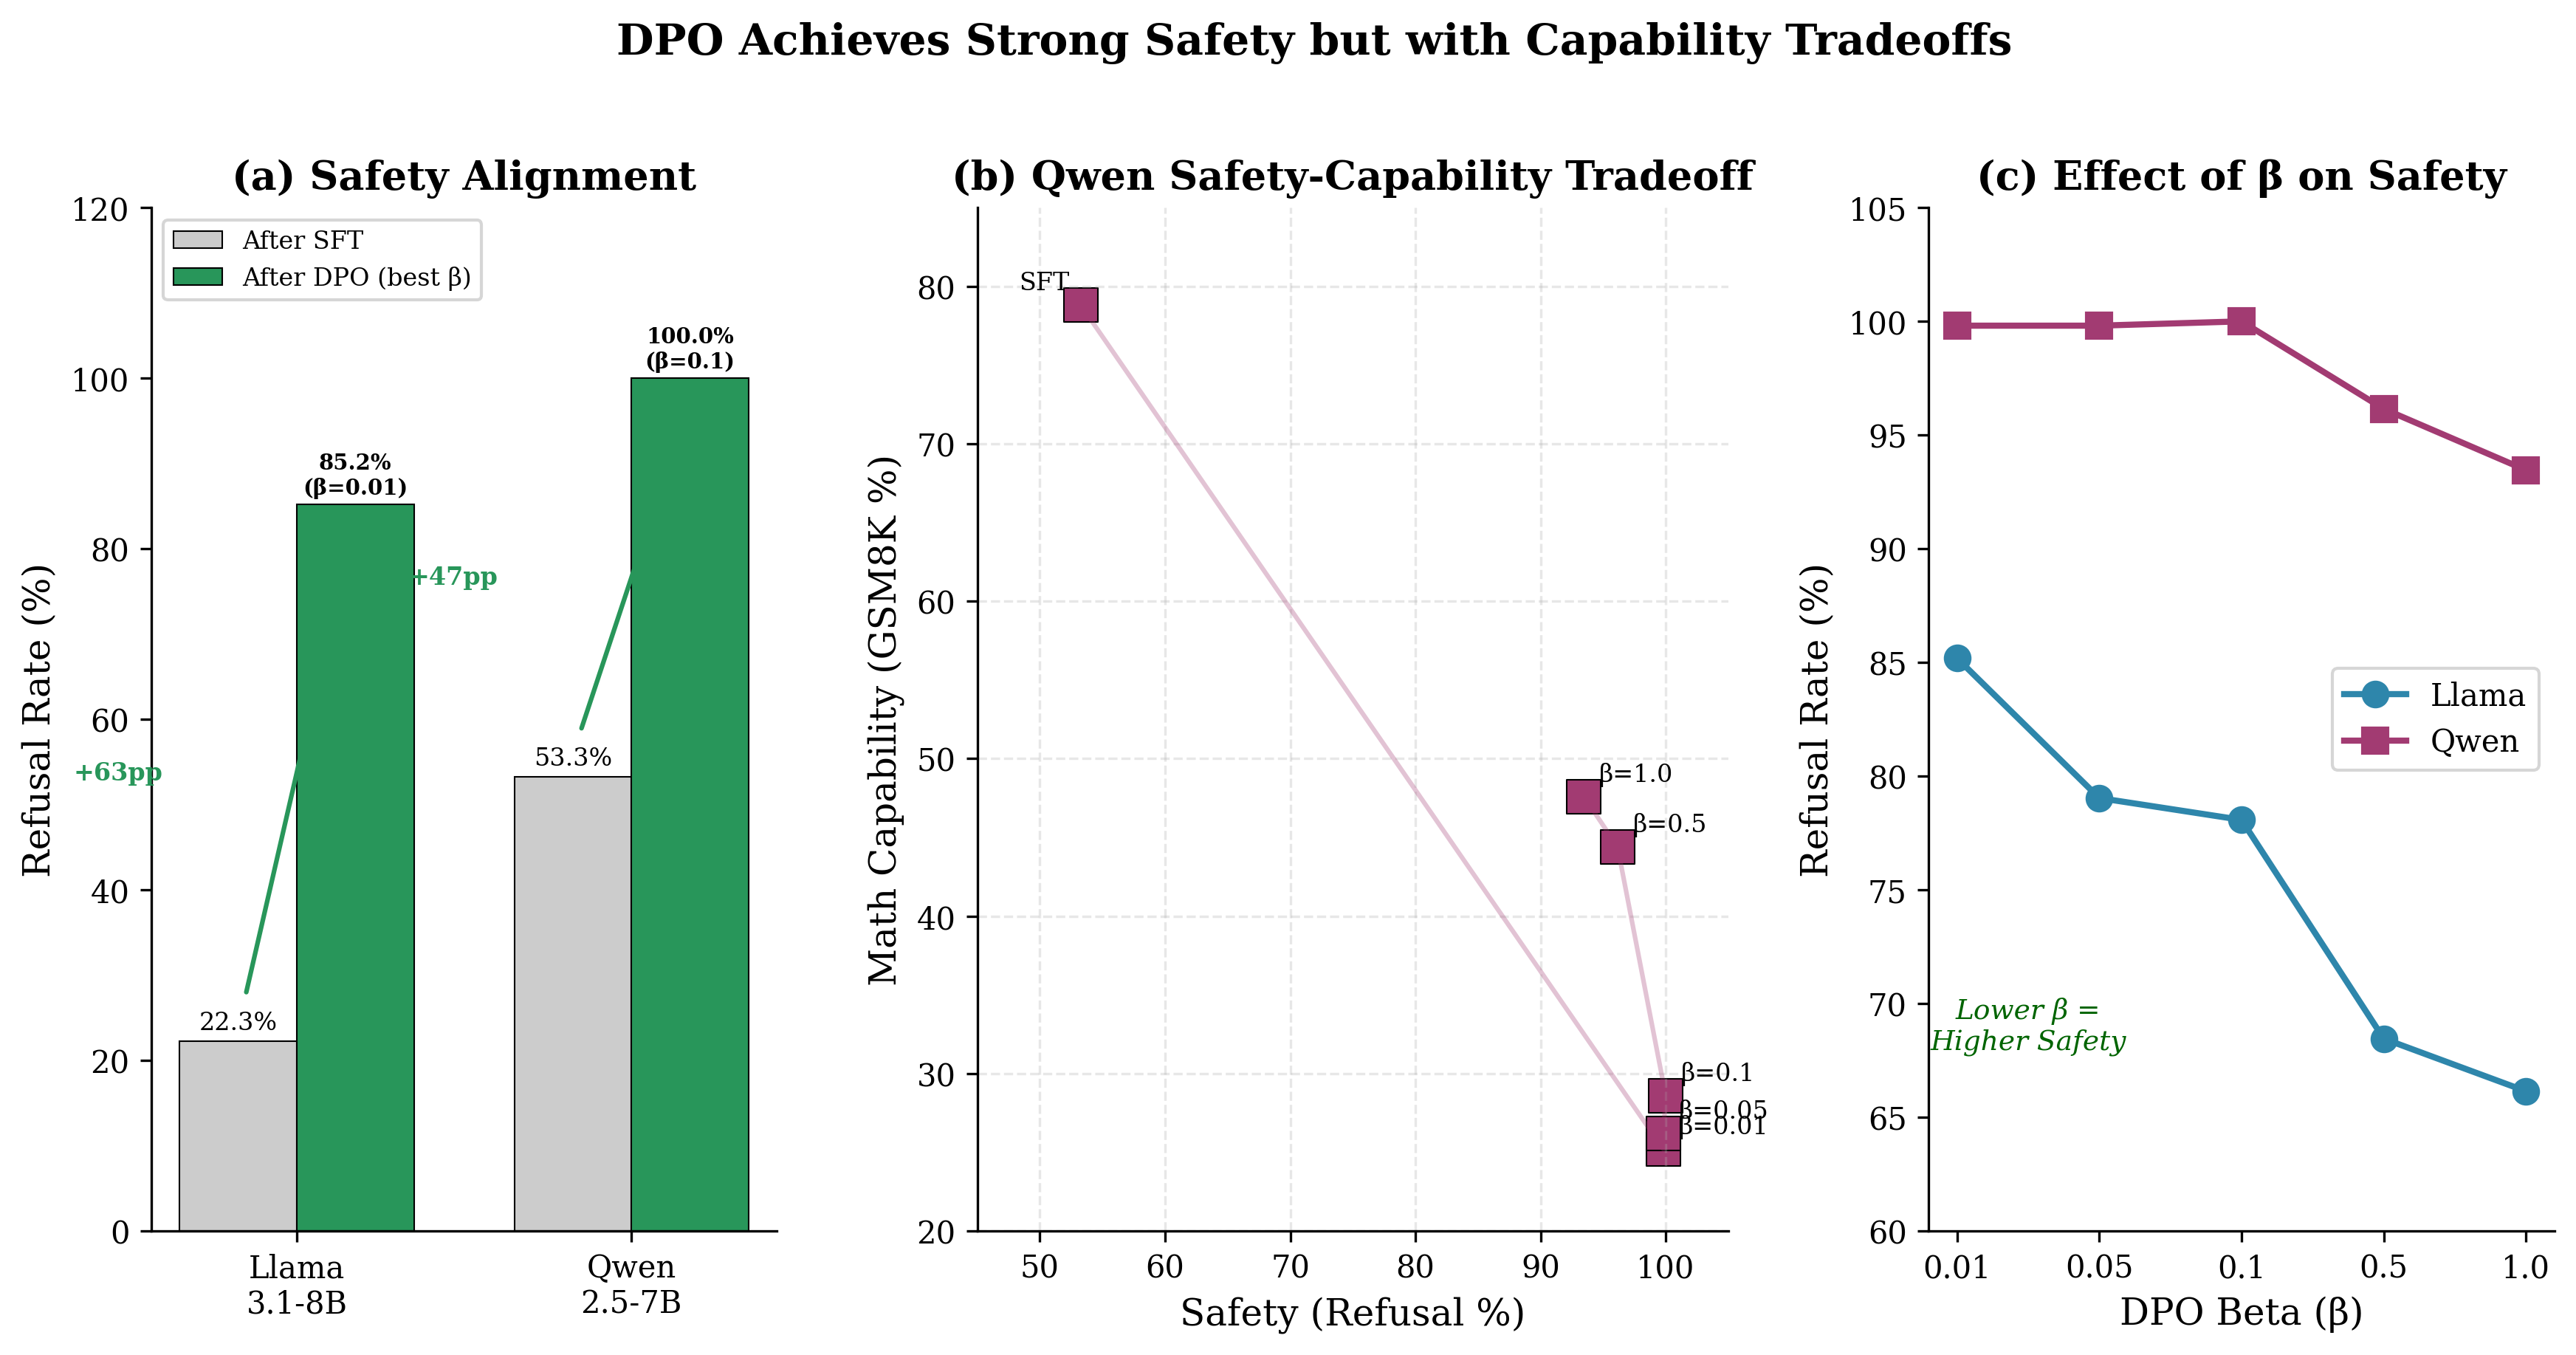
\includegraphics[width=\linewidth]{fig7_main_result.png}
    \caption{\textbf{Summary of the DPO safety--capability tradeoff.}
    (a) Safety improvements for both model families.
    (b) Qwen's safety--reasoning tradeoff (GSM8K vs.\ refusal), showing that GSM8K collapses
        as safety increases, with partial recovery at higher $\beta$.
    (c) Effect of $\beta$ on safety for both models.}
    \label{fig:summary}
\end{figure}

\subsection{A Tale of Two Models}

Llama 3.1-8B and Qwen 2.5-7B begin with markedly different safety profiles:
after SFT, Llama refuses only 22.3\% of AdvBench prompts, while Qwen refuses 53.3\%.
This highlights the influence of pretraining choices and built-in safety priors.
After applying DPO with the same filtered safety preference dataset, both models can
be moved into a 90--100\% refusal regime, demonstrating that preference-based
alignment is effective at shifting safety posture regardless of the starting point.

The key divergence lies in how capabilities respond to this shift.
Llama's performance on both MMLU and GSM8K remains stable across all $\beta$ values,
suggesting that for this architecture, DPO largely preserves the underlying reasoning
and knowledge circuits.
Qwen, however, suffers a dramatic loss in GSM8K accuracy when pushed toward
aggressive safety: a more than 50-point drop at low $\beta$, with only partial
recovery at higher regularization.
This difference indicates that the impact of DPO is \emph{model-dependent},
and that pretrained internal structure can modulate sensitivity to preference-based
alignment.

\subsection{Revisiting the Safety--Capability Tradeoff}

Our findings challenge simplified narratives about safety alignment.
DPO does not universally preserve capability, nor does it universally degrade it.
Instead, its effects are structured along three dimensions—the model family, the
task, and the alignment strength.

Under DPO with high-quality safety preferences, we observe that:
\begin{itemize}
    \item Safety gains of 40--60 percentage points are achievable across models.
    \item Factual knowledge (MMLU) remains consistently stable in all settings.
    \item Llama's reasoning (GSM8K) remains near its SFT baseline across the entire sweep.
    \item Qwen's reasoning is highly sensitive to alignment strength, collapsing at low
          $\beta$ and recovering only partially at higher values.
\end{itemize}

Thus, the capability tax is not a single scalar quantity.
There is \emph{no} catastrophic tradeoff along the knowledge axis, but there is a
substantial and model-specific tradeoff along the reasoning axis.
In this sense, the safety--capability frontier is multidimensional: a configuration
that appears ``free'' in the MMLU dimension may incur a severe cost in GSM8K.

\subsection{Practical Guidance and Limitations}

These findings suggest several practical guidelines for safety alignment with DPO.
First, clean and explicitly safety-focused preference data are essential for avoiding
unintended stylistic or helpfulness effects.
Second, $\beta$ should be tuned with awareness of downstream task demands:
aggressive alignment maximizes refusal rates but can greatly impair multi-step
reasoning, particularly for certain model architectures.
Finally, practitioners should evaluate safety and capability along multiple axes
rather than relying on a single aggregate score.

Our study has limitations.
Although our evaluation is larger in scope than prior work, the sample sizes used
(520 AdvBench, 1{,}000 MMLU, 500 GSM8K per configuration) remain moderate.
We also examine only one alignment algorithm (DPO) and one safety preference
dataset (PKU-SafeRLHF); other preference sources or alignment methods may yield different
tradeoff structures, and our findings may not generalize to all safety datasets.
Finally, our analysis is behavioral: we do not study changes in internal
representations or the geometry of parameter updates, which represent important
directions for mechanistic follow-up work.

% -------------------------------------------------------------
\section{Future Work}
\label{sec:future_work}

Our original proposal aimed not only to characterize the behavioral
safety--capability tradeoff, but also to investigate its \emph{geometric}
underpinnings. While the present study focuses on external evaluations,
future work will extend this analysis into the representation space of
safety-aligned models. Several directions appear especially promising.
First, studying geometric quantities such as safety-direction strength,
feature subspace rank, and decision-boundary margin may help explain why
Qwen's reasoning abilities are disproportionately affected by aggressive
alignment while Llama remains stable. Second, geometric diagnostics could
enable prediction of over-refusal---and more generally, capability
degradation---\emph{before} behavioral evaluation, offering a principled tool
for selecting alignment strength. Finally, connecting preference-based
updates to mechanistic changes in internal circuits may deepen our
understanding of why safety alignment induces over-generalization in some
architectures but not others. We view this geometric analysis as a natural
and important next step toward a unified theory of the safety--reasoning
tradeoff in aligned LLMs.


% -------------------------------------------------------------
\section{Conclusion}
\label{sec:conclusion}

We set out to examine whether safety alignment via DPO inevitably incurs a capability
tax, or whether models can be made substantially safer while preserving their general
abilities. Our results provide a nuanced answer. Using strictly filtered safety
preferences across two distinct model families, we find that DPO reliably delivers
large safety gains—40--60 percentage points on AdvBench—without degrading factual
knowledge, as measured by MMLU. For Llama 3.1-8B, even multi-step reasoning on GSM8K
remains stable across all alignment strengths, demonstrating that safety alignment
need not compromise core capabilities.

For Qwen 2.5-7B, however, aggressive alignment induces a pronounced reasoning-specific
capability tax: GSM8K accuracy collapses under low $\beta$ and recovers only partially
under stronger regularization. This contrast highlights that the safety--capability
tradeoff is not monolithic but depends on the interaction between model architecture,
task type, and alignment strength. In this sense, capability preservation is not a
guaranteed property of safety alignment, but neither is capability loss inevitable.

Taken together, our findings point toward a structured and model-dependent
safety--reasoning tradeoff. They emphasize the importance of evaluating alignment
methods along multiple capability axes and tuning alignment strength with downstream
task requirements in mind. Combined with the geometric directions outlined in
Section~\ref{sec:future_work}, our results offer a foundation for developing more
predictive and principled approaches to safety alignment in large language models.

% -------------------------------------------------------------
\bibliographystyle{plainnat}
\begin{thebibliography}{99}

\bibitem{dpo}
R.~Rafailov, A.~Sharma, E.~Mitchell, et al.
\newblock Direct Preference Optimization: Your Language Model is Secretly a Reward Model.
\newblock \url{https://arxiv.org/abs/2305.18290}

\bibitem{pku-saferlhf}
J.~Ji, D.~Hong, B.~Zhang, et al.
\newblock PKU-SafeRLHF: Aligning Large Language Models with Safe Reinforcement Learning from Human Feedback.
\newblock \url{https://arxiv.org/html/2406.15513v3}

\bibitem{rlhf}
P.~Christiano, J.~Leike, T.~Brown, et al.
\newblock Deep reinforcement learning from human preferences.
\newblock \url{https://arxiv.org/abs/1706.03741}


\bibitem{llama3}
Meta AI.
\newblock The Llama 3 Herd of Models.
\newblock \url{https://arxiv.org/abs/2407.21783}

\bibitem{qwen2.5}
Alibaba Cloud.
\newblock Qwen2.5 Technical Report.
\newblock \url{https://arxiv.org/abs/2412.15115}

\bibitem{advbench}
A.~Zou, Z.~Wang, N.~Carlini, M.~Nasr, J.~Kolter, M. ~Fredrikson.
\newblock Universal and transferable
adversarial attacks on aligned language models
\newblock \url{https://arxiv.org/abs/2307.15043}

\bibitem{mmlu}
D.~Hendrycks, C.~Burns, S.~Basart, et al.
\newblock Measuring Massive Multitask Language Understanding
\newblock \url{https://arxiv.org/abs/2009.03300}

\bibitem{gsm8k}
K.~Cobbe, V.~Kosaraju, M.~Bavarian, et al.
\newblock Training Verifiers to Solve Math Word Problems.
\newblock \url{https://arxiv.org/abs/2110.14168}

\bibitem{llm-overrefusal}
J.~Zhang, R.~Chen, et al.
\newblock Understanding and Mitigating Over-refusal for Large Language Models via Safety Representation
\newblock \url{https://arxiv.org/html/2511.19009v1}

\bibitem{askell2021alignment}
A.~Askell, Y.~Bai, A.~Chen, et al.
\newblock A General Language Assistant as a Laboratory for Alignment.
\newblock \url{https://arxiv.org/abs/2112.00861}

\bibitem{orbench}
J.~Cui, W.~Chiang, I.~Stoica, C.~Hsieh.
\newblock OR-Bench: An Over-Refusal Benchmark for Large Language Models
\newblock \url{https://arxiv.org/html/2405.20947}

\bibitem{falsereject}
Z.~Zhang, W.~Xu, F.~Wu, C.~Reddy.
\newblock FalseReject: A Resource for Improving Contextual Safety and Mitigating Over-Refusals in LLMs via Structured Reasoning
\newblock \url{https://arxiv.org/abs/2505.08054}

\end{thebibliography}
\end{document}
